\section{Introduction}
\label{sec:intro}
Partial observability is a core challenge for robot manipulation~\cite{Zare2024Survey,Zhu2025Point}.
Visual observations are partial projections of a 3D scene from limited viewpoints, so task-relevant information can be missing from the current input~\cite{Jangir2022Look,Akinola2020Learning,Yan2018Grasping}.
When the missing regions contain object parts, support relations, contact surfaces, or actionable regions, the problem is not simply perceptual noise.
It becomes structural incompleteness, where the policy must act using scene structure that is only partially observed.

Existing visuomotor imitation learning methods improve scene understanding with richer representations, including object-centric representations that focus on task-relevant objects~\cite{zhu2022viola,zhu2023learning,Qian2024SOFT,Shi2024Composing,Qian2024Task} and structured representations such as keypoints, semantic fields, and geometric abstractions~\cite{Chen2021Unsupervised,Wang2025GenDP,Yang2025GravMAD,Simeonov2022Neural,Ryu2024EDFS}.
However, these representations are still largely derived from visible observations.
They can make observed cues easier to use, but they do not explicitly model how visible evidence constrains unseen object structure.
As illustrated in fig.~\ref{fig:intro}, this limitation can make traditional imitation learning ambiguous and brittle when successful manipulation depends on hidden supports, physical relations, or spatial arrangements.

\begin{figure}[t]
    \centering
    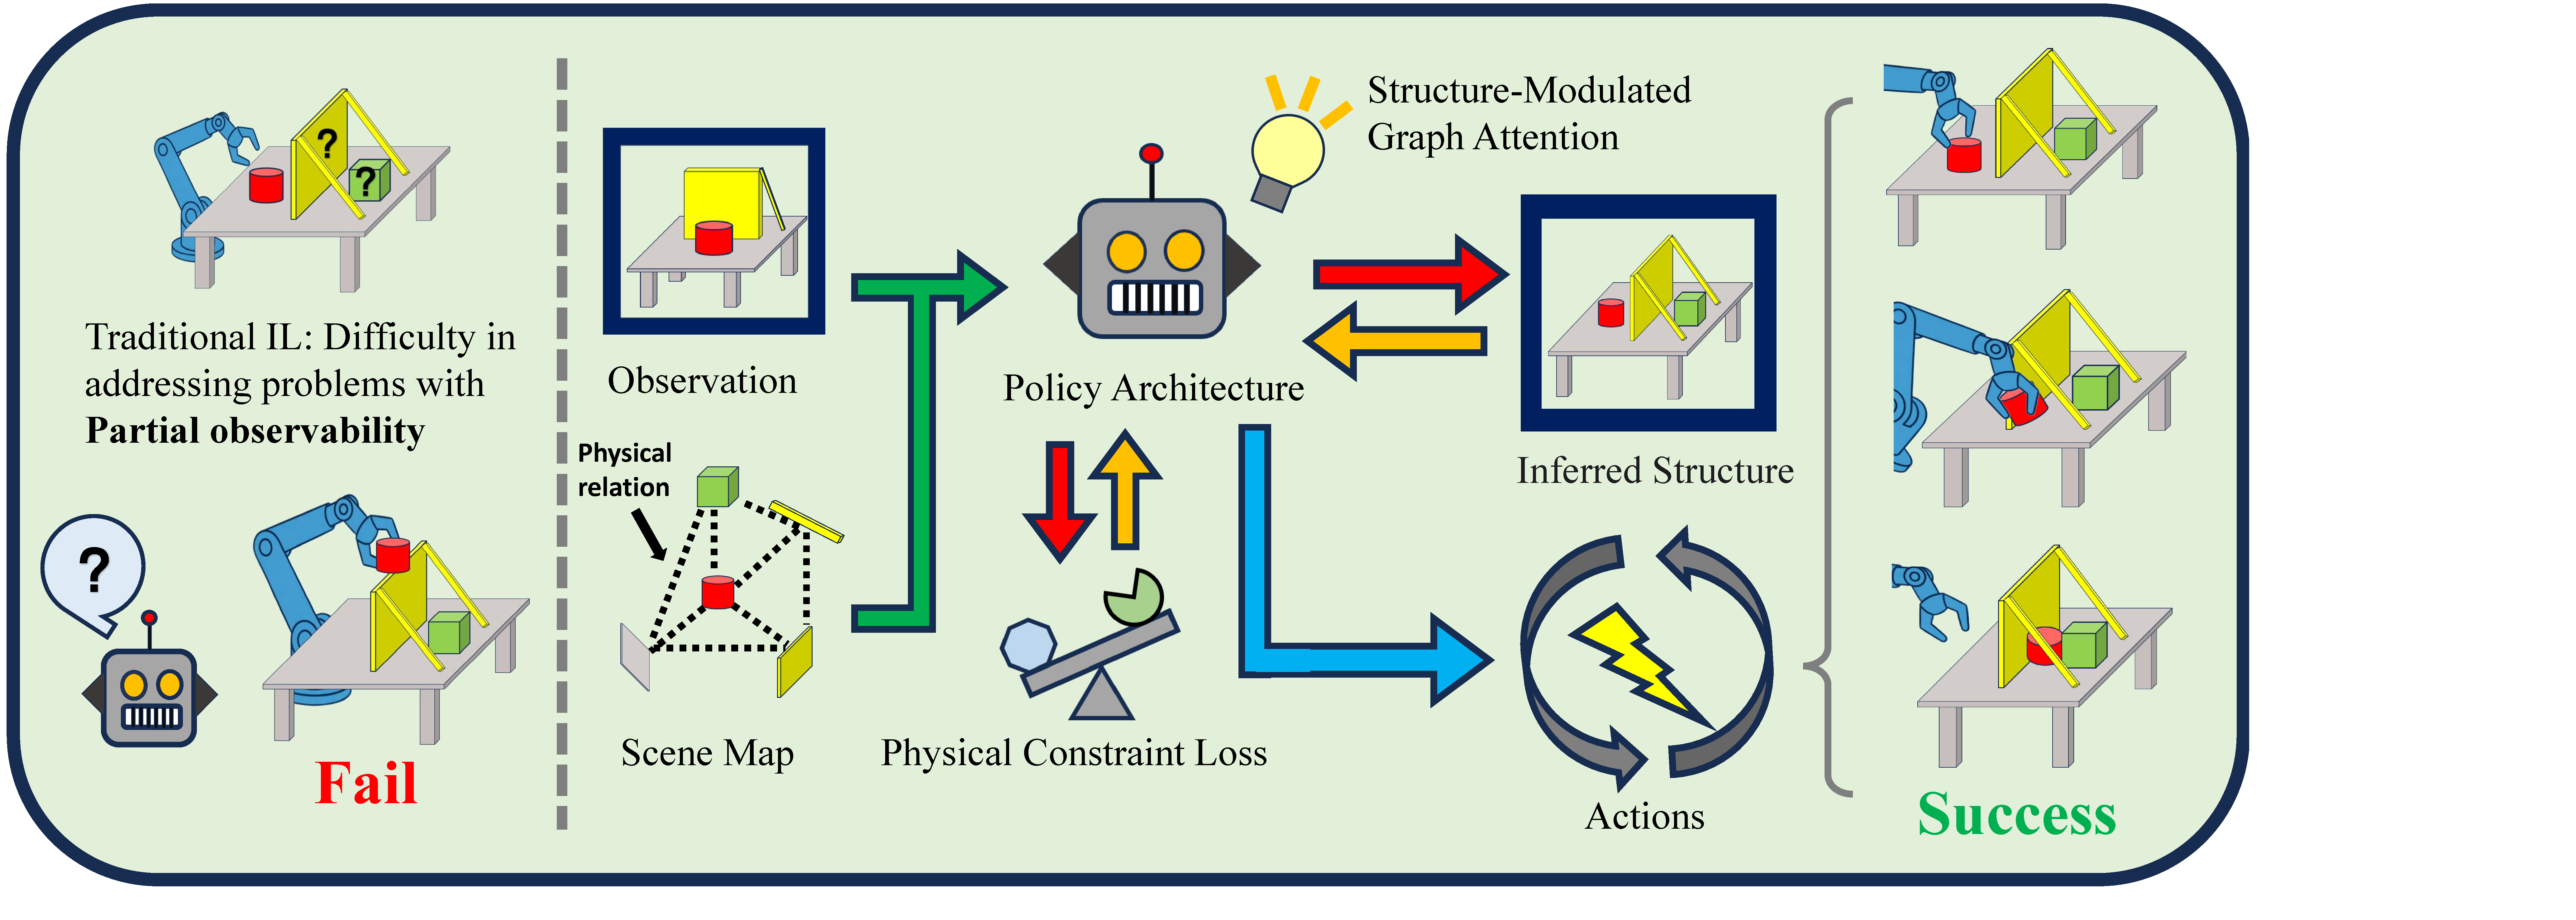
\includegraphics[width=0.85\linewidth]{figs/intro.pdf}
    \caption{Overview of MapPolicy. Traditional imitation learning can fail under partial observability because the current observation omits task-relevant structure. MapPolicy augments the observation with a Scene Map that captures physical relations, uses structure-modulated graph attention to infer hidden structure, and regularizes learned features with physical constraint loss for action prediction.}
    \label{fig:intro}
\end{figure}

Humans are often more robust in similar situations because they use prior knowledge of object structure and physical relations to infer what is not visible.
For example, when placing an object onto a shelf, a person does not need to see every layer of the shelf to infer the existence and approximate position of supporting surfaces.
This observation suggests that robust manipulation under partial observability requires more than stronger encoding of visible pixels or point clouds.
It requires a representation that exposes object structure and physical relations as explicit priors, consistent with the view that affordance and action are grounded in environmental structure~\cite{Gibson1979TheEA}.

To this end, we propose Scene Map, a structured scene representation for policy learning.
Scene Map represents a manipulation scene as a graph of geometric primitives and physical relations.
Nodes describe primitive-level object parts such as cuboids and cylinders through their shape, scale, 3D position, and rotation, while edges encode connectivity and physical constraints between primitives.
This design follows work on hierarchical graphs, part decompositions, and compositional geometric primitives~\cite{Mo2019StructureNet,Tulsiani2016LearningSA,Zou20173DPRNNGS,Paschalidou2019SuperquadricsRL,Paschalidou2020LearningUH,Sun2025ConceptFactory}.
By organizing object shape, part structure, spatial layout, and constraints in a graph, Scene Map provides structural cues that are not reliably available from the current observation alone.

Building on Scene Map, we introduce MapPolicy, an imitation learning framework that fuses map features with visual and robot state features for action prediction.
MapPolicy uses Structure-Modulated Graph Attention to propagate global structural and spatial information through primitive features, allowing visible parts and physical relations to inform the representation of hidden components.
It also uses Physical Constraint Loss to regularize learned map features with geometric and kinematic consistency.
Together, these components help the policy infer task-relevant structure from partial observations and use the inferred structure for manipulation.

We evaluate MapPolicy on 49 simulation tasks across MetaWorld, RLBench, and ManiSkill, together with five real-world tasks.
Across these settings, MapPolicy consistently improves over visual, diffusion-based, and 3D policy baselines on articulated interaction, contact-rich control, and precise spatial arrangement.

Our contributions can be summarized as follows:
\textbf{(1)} We tackle partial observability by introducing Scene Map as a structural scaffold that models object shape, part structure, spatial layout, and physical constraints.
By turning occluded but task-relevant structure into prediction targets and constraining these predictions with physical relations, Scene Map provides the policy with cues for inferring unseen components from partial observations.
\textbf{(2)} We propose MapPolicy, a policy framework that incorporates Scene Map into imitation learning by integrating structured scene representations with visual and robot state observations.
\textbf{(3)} We design two mechanisms that make structural priors effective for policy learning: Structure-Modulated Graph Attention for propagating global structural and spatial information through primitive features, and Physical Constraint Loss for enforcing geometric and kinematic consistency in learned map features.
\textbf{(4)} We conduct comprehensive evaluations across 49 simulation tasks in MetaWorld, RLBench, and ManiSkill, together with five real-world tasks, demonstrating consistent performance gains in partial-observability, articulated-interaction, contact-rich manipulation, and precise spatial-arrangement settings.
